\section{Introduzione}
In questo capitolo si vuole capire quali potenzialità
la piattaforma di Erlang/Elixir porta, in modo da poter
capire quali siano le applicazioni possibili con questa tecnologia.

Vogliamo capire i casi d'uso di questa tecnologia, attraverso una serie
di test empirici e provare a fare qualche confronto con altri
linguaggi.

% ---------------------Hardware utilizzato-------------------------- 
\subsection{Hardware utilizzato}

I test vengono eseguiti sul sistema operativo linux, viene riportato in
figura \ref{fig:neofetch} l'output del tool \textbf{neofetch} che riporta
le caratteristiche del computer utilizzato per l'esecuzione dei test,
in particolare notiamo che la CPU di riferimento dei test
ha 8 core logici e 4 fisici, e di default la VM alloca 8 scheduler,
uno per ogni core logico.

\begin{figure}[!htp]
    \centering
    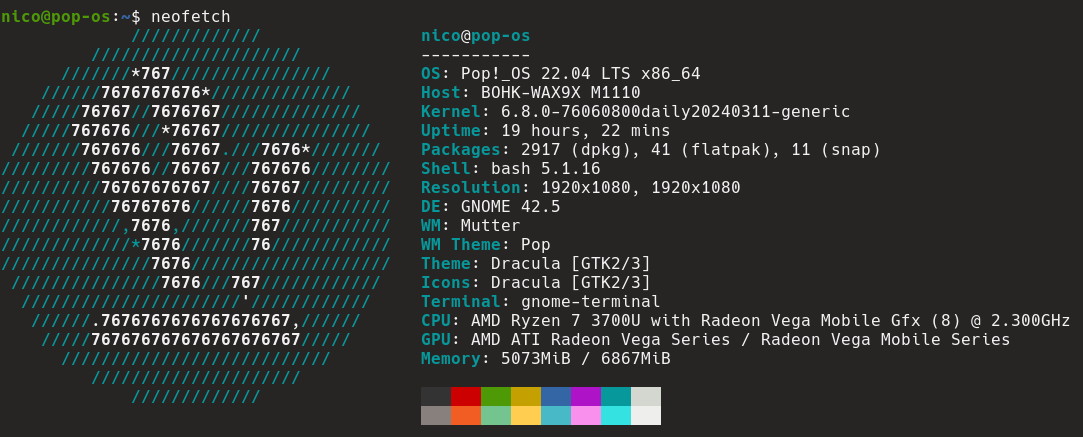
\includegraphics[keepaspectratio=true,scale=0.33]{images/neofetch.png}
	\caption{Hardware computer utilizzato}
  	\label{fig:neofetch}
\end{figure}

% ---------------------Test Interoperabilità-------------------------- 


